% Rewrite of existing lab manual: Lenses and Mirrors
% Institute for Physics and Astronomy
% University of Alabama
% Authors:
% - mknipfer
% - aghadimi
% Date: 07.12.2019

\documentclass[11pt, a4paper]{article} 

\input{structure.tex} % Specifies the document structure and loads requires packages
\title{Lenses and Mirrors}
\date{}
\author{}
\institution{Department of Physics and Astronomy, University of Alabama}

\begin{document}

% ---- Title stuff -----------------------
\thispagestyle{empty}
\noindent
\begin{tabularx}{\textwidth}{ll>{\raggedleft\arraybackslash}Xr}
    Course and Section: & \underline{\hspace{2cm}} & Names: & \underline{\hspace{6cm}}\\[0.3cm]
    Date: & \underline{\hspace{2cm}} & & \underline{\hspace{6cm}}\\[0.3cm]
    & & TA name: & \underline{\hspace{6cm}}
\end{tabularx}
\bigskip
\begin{center}
    {\Huge \bf Lenses and Mirrors}\\
\end{center}
% ----------------------------------------
\begin{center}
\textsc{Answer all questions from the text on the lines beneath.}
\end{center}
In this experiment you will study lenses and mirrors by creating images on screens.
By doing so you will study the laws describing them.

\section{Equipment}
\begin{minipage}{0.49\textwidth}
    \begin{itemize}
        \item Optical bench
        \item Converging lens, diverging lens
        \item Light source (as an object)
    \end{itemize}
\end{minipage}
\begin{minipage}{0.49\textwidth}
    \begin{itemize}
        \item Viewing screen
        \item Mirror
        \item Half-screen
    \end{itemize}
\end{minipage}

\section{Procedure}
\subsection{Converging lens}
Take a \textit{converging lens} and examine it.
Is it thicker or thinner in the center?
What do objects look like through it?
Could it be used as a magnifying glass?
Try the lens both close to objects and far away.
\fillwithlines{3cm}
If a lens is used to form an image of something infinitely far away, the
distance from the lens to the image is defined to be the focal length. 
This is because the rays from an infinitely remote object are essentially
parallel (to the optical axis) and thus converge at the \textit{focal point} $f$.
The distance from the lens axis to the focal point is called the
\textit{focal length}.

Use the lens to form an image of “something far away”. 
To do this, place the lens on the optical bench and move the screen on the
bench until a sharp image is formed on it. 
\begin{figure}[tbh]
    \centering
    \def\svgwidth{\textwidth}
    \input{figures/convergingLens.pdf_tex}
    \caption{Converging lens: For an object outside of the focal point a \textit{real}
    inverted image is formed.}
    \label{fig:convLens}
\end{figure}
\begin{equation*}
    \text{Focal length} = \underline{\hspace{2cm}}\si{cm}
\end{equation*}

The equation relating the image and object distances of a \textit{thin lens} is
\begin{equation}
    \frac{1}{p} + \frac{1}{q} = \frac{1}{f}\,.
    \label{eq:f}
\end{equation}

\subsection{Image-Object Relationship of a Converging Lens}
In this part, use the light box as the object; the lens will form an image of
this box on the screen.
Place the object and the screen at opposite ends of the bench such that the
distance between them is 110 cm.
Place a white sheet of paper in front of the white screen. 
Move the lens between them until a sharp image is formed on the screen.
You should note that there are two positions for the lens which give sharp
images. \textit{Why} is that so?
\fillwithlines{3cm}

Take measurements for each of these positions.
Repeat these measurements for $L = 100~\si{cm}$ and $L = 90~\si{cm}$.
Record the distance $p$ from the lens to the object and the distance
$q$ from the lens to the image.
Also measure the height $h'$ of the image and the height $h$
of the object.
\begin{equation*}
    h = \underline{\hspace{2cm}}\si{cm}
\end{equation*}

\begin{center}
    \def\arraystretch{1.5}
    \setlength\tabcolsep{0.6cm}
    \begin{tabular}{|c|c|c|c|c|c|c|}
        \hline
        \rowcolor{gray!40}
        $L$ (cm) & $p$ (cm) & $q$ (cm) & $h'$ (cm) & $f$ (cm) & $h'/h$ & $q/p$ \\
        \hline
        110 & ~ & ~ & ~ & ~ & ~ & ~ \\
        \hline
        110 & ~ & ~ & ~ & ~ & ~ & ~ \\
        \hline
        100 & ~ & ~ & ~ & ~ & ~ & ~ \\
        \hline
        100 & ~ & ~ & ~ & ~ & ~ & ~ \\
        \hline
        90 & ~ & ~ & ~ & ~ & ~ & ~ \\
        \hline
        90 & ~ & ~ & ~ & ~ & ~ & ~ \\
        \hline
    \end{tabular}
\end{center}

Use equation~(\ref{eq:f}) to calculate the \textit{focal length} $f$ from each set of data in the table
and fill in that part of the table.
What $f$, $p$ and $q$ are is also shown in figure~\ref{fig:convLens}.
\begin{itemize}
    \item Do you get consistent values for the \textit{focal length} $f$?
    \item Do these results agree with the focal length you found in the \textit{first part} of the experiment?
    \item Which method do you think is the most \textit{accurate}?
\end{itemize}
\fillwithlines{3cm}
Finally, look at the \textit{last two columns} of the table.
Do you find that the two ratios are equal?
If so, why?
\fillwithlines{3cm}
\subsection{Diverging Lens}
A diverging lens will produce a virtual image of a real object. 
To observe this, place the lens on the optical bench about 20 cm from the light
box.
Move the screen on the bench, can you find the image on the screen?
Now, look at the light box through the lens, can you see the image?
\begin{itemize}
    \item Is this image smaller or bigger than the object?
    \item Is the image you are viewing \textit{inverted}?
    \item Is it \textit{virtual}?
    \item Is it located in \textit{front} or in the \textit{back} of the lens?
\end{itemize}
\fillwithlines{3cm}

\begin{figure}[tbh]
    \centering
    \def\svgwidth{0.7\textwidth}
    \input{figures/divergingLens.pdf_tex}
    \caption{The diverging lens creates a virtual image which we cannot capture on a screen.
    Thus we have to add a converging lens.}
    \label{fig:divLens}
\end{figure}

\begin{figure}[tbh]
    \centering
    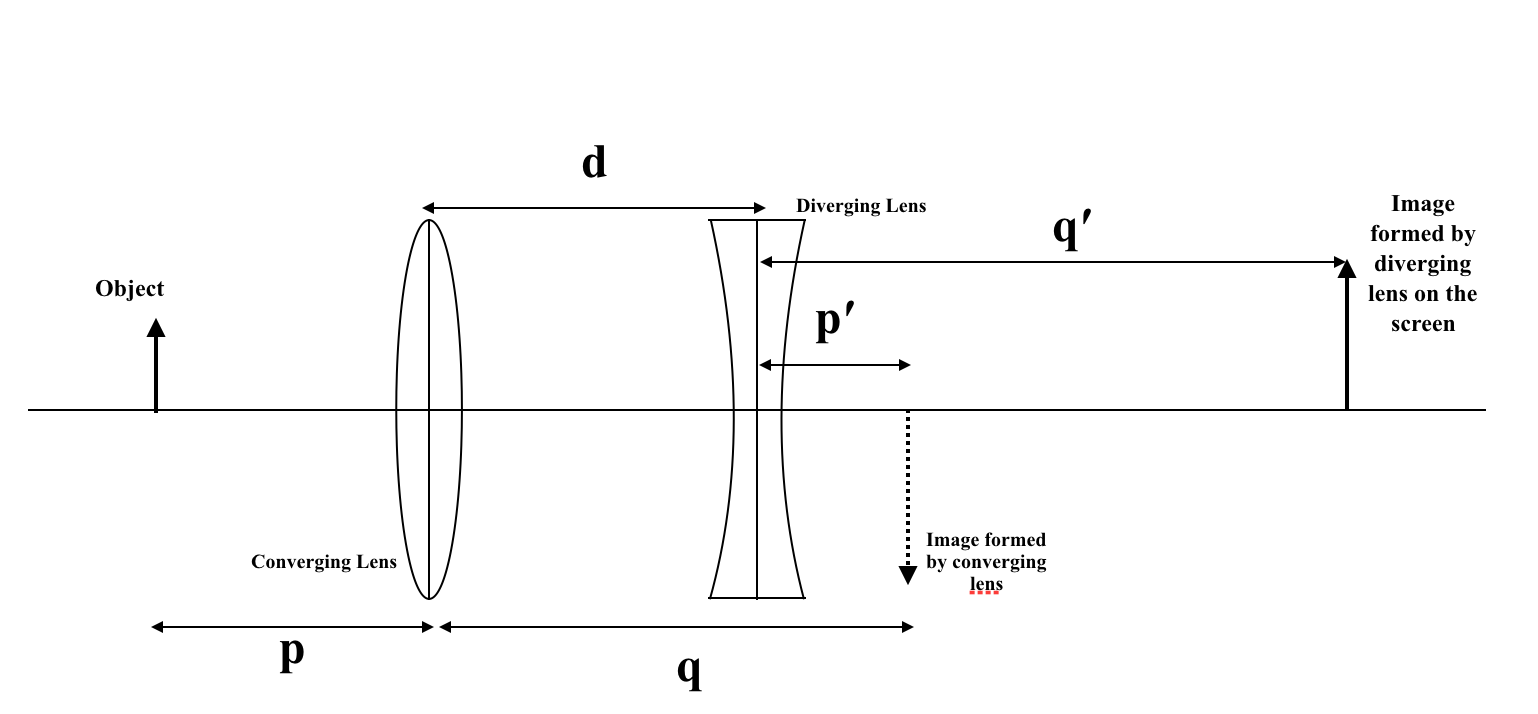
\includegraphics[width=\textwidth]{figures/ConvergingDivergingLens.png}
    \caption{A converging followed by a diverging lens.
    This way an upright real image is formed that can be captured on a screen.}
    \label{fig:divergingConvergingLens}
\end{figure}
In order to produce a real image by a diverging lens you also need to use a converging lens,
see figure~\ref{fig:divergingConvergingLens}.

\begin{enumerate}
    \item Start by forming a clear image on the screen using only the converging lens. Find the distance of the object to the lens p.
        Using the thin lens equation, calculate distance of the image q formed by the converging lens
        \begin{equation*}
            q = \underline{\hspace{2cm}} \si{cm}\,.
        \end{equation*}

    \item Insert the diverging lens between the image and the converging lens. Refer to the diagram for help.\\
    \item Measure the distance $d$ between the two lenses.
        \begin{equation*}
            d = \underline{\hspace{2cm}} \si{cm}\,.
        \end{equation*}
        The image created by the converging lens becomes the object for the diverging lens.
    \item Move the diverging lens until a real image is produced on the screen.
    \item Measure the ``new'' object distance $p'$, with respect to the diverging lens. Take the difference between the two distances $q$ and $d$.
        \begin{equation*}
            p' = q - d  = \underline{\hspace{2cm}} \si{cm}\,.
        \end{equation*}
    \item Measure the distance $q'$ between the screen and the diverging lens
        \begin{equation*}
            q'  = \underline{\hspace{2cm}} \si{cm}\,.
        \end{equation*}
    \item Finally, find the focal length of the diverging lens using the thin lens equation for $p'$, $q'$ and $f'$.
        \textit{Note:} In equation~(\ref{eq:fprime}) \textit{the sign} of $p'$ has to be negative, since the image formed by the converging lens is behind the diverging lens.
        \begin{equation}
            \frac{1}{p'} + \frac{1}{q'} = \frac{1}{f'}\,.
            \label{eq:fprime}
        \end{equation}
        Find the focal length $f'$ of the diverging lens,
        \begin{equation*}
            f'  = \underline{\hspace{2cm}} \si{cm}\,.
        \end{equation*}
\end{enumerate}


\end{document}
